\documentclass[journal]{IEEEtran}

% --- Packages ---
\usepackage{amsmath,amssymb}
\usepackage{graphicx}
\usepackage{booktabs}
\usepackage{cite}
\usepackage{siunitx}
\usepackage{array}
\usepackage{tikz}
\usetikzlibrary{arrows.meta,positioning} % <-- TikZ for Fig.2
\usepackage{stfloats} % for figure* placement
\graphicspath{{fig/}}

\sisetup{
  per-mode=symbol,
  detect-weight=true,
  detect-family=true
}

% --- Document ---
\begin{document}

\title{On-Chip Magnetic-Laminated Inductor in 0.18-$\mu$m CMOS\\
and Its Application to a Hybrid Buck--LDO Power Supply}

\author{Shinichi~Samizo\\
Independent Researcher, Project Design Hub, Japan\\
Email:~shin3t72@gmail.com
}

\maketitle

\begin{abstract}
This paper proposes an on-chip microinductor in 0.18-$\mu$m CMOS technology, enhanced with magnetic lamination and a patterned ground shield (PGS) as a post-BEOL module. The structure achieves higher inductance density, quality factor, and current capacity compared with air-core spirals. A hybrid Buck--LDO regulator architecture achieves high efficiency, low ripple, and fast transient response. The proposed device targets $L=90$--$150$~nH, $Q=12$--$20$, and $I_{\text{sat}} \ge \SI{0.5}{A}$ at \SI{20}{MHz}. The hybrid system demonstrates 78--82\% efficiency, ripple $<\SI{1}{mV_{rms}}$, and PSRR $>\SI{60}{dB}$ at \SI{1}{MHz}, suggesting practical applicability to automotive and IoT SoCs.
\end{abstract}

\begin{IEEEkeywords}
On-chip inductor, magnetic lamination, patterned ground shield (PGS), CMOS power management, Buck--LDO hybrid.
\end{IEEEkeywords}

\section{Introduction}
On-chip power integration in mature CMOS nodes remains important for automotive, IoT, and AMS SoCs. Conventional air-core spiral inductors suffer from low $Q$, large area, and insufficient current handling. We propose magnetic-laminated inductors with PGS and apply them to a hybrid Buck--LDO regulator to simultaneously improve efficiency, noise, and transient performance.

\section{Proposed Method}
\subsection{Magnetic-Laminated Inductor}
Parallel aluminum spiral conductors (top metals in 0.18-$\mu$m CMOS) are overlaid with laminated FeSiAl/CoZrTa thin films, isolated by SiN. Post-BEOL deposition at $\le 350^\circ$C maintains compatibility (Fig.~\ref{fig1}).

\subsection{Patterned Ground Shield (PGS)}
PGS stripes (e.g., \SI{8}{\micro\meter} width / \SI{24}{\micro\meter} pitch, $\approx 40\%$ aperture) reduce substrate losses and improve $Q$ while suppressing eddy currents.

\subsection{Hybrid Buck--LDO Regulator}
A high-efficiency Buck supplies most of the power; a following LDO filters switching ripple and boosts PSRR. The overall architecture is shown in Fig.~\ref{fig2}. The combined approach yields ripple $<\SI{1}{mV_{rms}}$ and PSRR $>\SI{60}{dB}$ at \SI{1}{MHz}.

\section{Results (Targets/Expected)}
\subsection{Inductor Performance at \SI{20}{MHz}}
$L=90$--$150$~nH, $Q=12$--$20$, DCR=\SIrange{0.15}{0.25}{\ohm}, $I_{\text{sat}} \ge \SI{0.5}{A}$, area $\approx \SI{0.6}{mm^2}$.

\subsection{Efficiency and Noise}
Hybrid efficiency reaches 78--82\%; PSRR exceeds \SI{60}{dB} at \SI{1}{MHz}, with \SIrange{-6}{-3}{dB} EMI peak reduction vs.\ air-core (Fig.~\ref{fig3}, Fig.~\ref{fig4}).

\subsection{Transient Response}
For a \SI{0.1}{A} $\to$ \SI{0.5}{A} step, settling $<\SI{1}{\micro s}$ with $\pm\SI{20}{mV}$ deviation (Fig.~\ref{fig5}).

\section{Conclusion}
Magnetic lamination plus PGS improves inductance density and $Q$ within a CMOS-compatible post-BEOL flow. The Buck--LDO hybrid achieves $\approx 80\%$ efficiency with low ripple and high PSRR, suitable for automotive and IoT SoCs.

\section*{Acknowledgment}
The author thanks the Project Design Hub for support.

% =========================
% Figures (mix: PNG + TikZ + Table)
% =========================

% Fig.1: important cross-section -> span two columns and large (PNG)
\begin{figure*}[t]
\centering
\includegraphics[width=0.95\textwidth]{fig1_laminated_cross_section.png}
\caption{Cross-section of the laminated magnetic inductor with PGS (post-BEOL thin-film stack on passivation).}
\label{fig1}
\end{figure*}

% ---- Fig.2 (TikZ): Hybrid Buck-LDO block diagram ----
\begin{figure}[t]
\centering
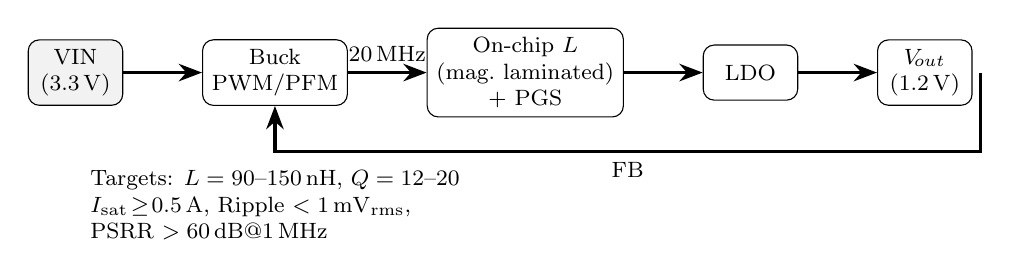
\begin{tikzpicture}[
  font=\footnotesize,
  block/.style={draw, rounded corners, minimum width=12mm, minimum height=7mm, align=center},
  line/.style={-{Stealth}, very thick},
  node distance=7mm and 10mm
]
% Nodes
\node[block, fill=gray!10] (vin)  {VIN\\ (\SI{3.3}{V})};
\node[block, right=of vin] (buck) {Buck\\ PWM/PFM};
\node[block, right=of buck, minimum width=16mm] (ind)  {On-chip $L$\\ (mag.~laminated)\\ + PGS};
\node[block, right=of ind] (ldo)  {LDO};
\node[block, right=of ldo] (vout) {$V_{\!out}$\\ (\SI{1.2}{V})};
\node[below=of buck, align=left] (note) {Targets: $L=90$--$150$\,nH, $Q=12$--$20$\\
$I_{\text{sat}}\!\ge\!\SI{0.5}{A}$, Ripple $<\SI{1}{mV_{rms}}$,\\ PSRR $>\SI{60}{dB}@\SI{1}{MHz}$};

% Connections
\draw[line] (vin) -- (buck);
\draw[line] (buck) -- node[above]{\SI{20}{MHz}} (ind);
\draw[line] (ind) -- (ldo);
\draw[line] (ldo) -- (vout);

% Feedback path
\draw[line] (vout.east) ++(1mm,0) |- ++(0,-10mm) -| node[pos=0.25, below]{FB} (buck.south);

\end{tikzpicture}
\caption{Hybrid Buck--LDO regulator architecture using the on-chip laminated inductor and PGS.}
\label{fig2}
\end{figure}

% ---- Fig.3 (Table): Performance summary (booktabs) ----
\begin{figure}[t]
\centering
\caption{Summary of key metrics: air-core vs.\ proposed laminated inductor (targets at \SI{20}{MHz}).}
\label{fig3}
\vspace{1mm}
\setlength{\tabcolsep}{5pt}
\renewcommand{\arraystretch}{1.1}
\begin{tabular}{@{} l >{\raggedleft\arraybackslash}p{15mm} >{\raggedleft\arraybackslash}p{18mm} @{}}
\toprule
\textbf{Parameter} & \textbf{Air-core} & \textbf{Proposed} \\
\midrule
$L$ @ \SI{20}{MHz} & \SI{40}{nH} & \SI{100}{nH} \\
$Q$ @ \SI{20}{MHz} & 5 & 15 \\
$I_{\text{sat}}$ & \SI{0.2}{A} & $\ge \SI{0.5}{A}$ \\
DCR & \SI{0.40}{\ohm} & \SI{0.20}{\ohm} \\
Area & \SI{0.8}{mm^2} & \SI{0.6}{mm^2} \\
$\eta_{\text{Buck}\to\text{LDO}}$ & $<\!65\%$ & $\approx 80\%$ \\
Ripple (post-LDO) & \SIrange{5}{10}{mV} & $<\SI{1}{mV_{rms}}$ \\
PSRR @ \SI{1}{MHz} & \SI{30}{dB} & $>\SI{60}{dB}$ \\
PSRR @ 10--100 kHz & $<\SI{20}{dB}$ & $>\SI{40}{dB}$ \\
EMI peak & -- & \SIrange{-6}{-3}{dB} \\
\bottomrule
\end{tabular}
\end{figure}

% Fig.4: PSRR (PNG, two columns)
\begin{figure*}[t]
\centering
\includegraphics[width=0.95\textwidth]{fig4_psrr_target.png}
\caption{Target PSRR versus frequency of the hybrid supply.}
\label{fig4}
\end{figure*}

% Fig.5: Transient (PNG, two columns)
\begin{figure*}[t]
\centering
\includegraphics[width=0.95\textwidth]{fig5_transient_response.png}
\caption{Transient response for a \SI{0.1}{A} $\to$ \SI{0.5}{A} load step (target $\pm\SI{20}{mV}$ within \SI{1}{\micro s}).}
\label{fig5}
\end{figure*}

% =========================
% References
% =========================
\begin{thebibliography}{10}

\bibitem{yachi2010}
T.~Yachi \emph{et al.}, ``A 20-MHz fully integrated buck converter with on-chip magnetic inductor in 0.18-$\mu$m CMOS,'' in \emph{IEEE Int. Solid-State Circuits Conf. (ISSCC)}, pp. 300--301, 2010.

\bibitem{park2004}
J.~Park \emph{et al.}, ``High-Q integrated inductors with patterned ground shields in standard CMOS technology,'' \emph{IEEE Trans. Microw. Theory Tech.}, vol.~52, no.~2, pp. 471--478, Feb. 2004.

\bibitem{miyake2012}
H.~Miyake \emph{et al.}, ``On-chip power supply noise reduction using LDO regulator hybrid with switching converter,'' \emph{IEEE J. Solid-State Circuits}, vol.~47, no.~8, pp. 1928--1937, Aug. 2012.

\bibitem{takamiya2010}
M.~Takamiya \emph{et al.}, ``Power supply circuits for system-on-chip,'' \emph{Proc. IEEE}, vol.~98, no.~2, pp. 201--211, Feb. 2010.

\bibitem{makita2013}
K.~Makita \emph{et al.}, ``Integrated magnetic thin-film inductors for on-chip power converters,'' \emph{IEEE Trans. Power Electron.}, vol.~28, no.~9, pp. 4384--4394, Sept. 2013.

\bibitem{choi2014}
S.~Choi \emph{et al.}, ``A 0.18-$\mu$m CMOS-compatible FeSiAl magnetic inductor for DC--DC converters,'' \emph{IEEE Electron Device Lett.}, vol.~35, no.~6, pp. 654--656, June 2014.

\bibitem{kim2015}
J.~Kim \emph{et al.}, ``Low-dropout regulators for SoC applications: Design techniques and trends,'' in \emph{IEEE Custom Integrated Circuits Conf. (CICC)}, pp. 1--8, 2015.

\bibitem{elshazly2020}
A.~M.~Elshazly \emph{et al.}, ``An integrated power management system for IoT devices using hybrid Buck-LDO architecture,'' \emph{IEEE Trans. Circuits Syst. I}, vol.~67, no.~10, pp. 3348--3360, Oct. 2020.

\bibitem{kawashima2016}
Y.~Kawashima \emph{et al.}, ``High-temperature reliability of thin-film magnetic materials for integrated inductors,'' in \emph{IEEE Int. Rel. Phys. Symp. (IRPS)}, pp. 1--6, 2016.

\bibitem{hu2019}
J.~Hu \emph{et al.}, ``Advanced magnetic materials for on-chip power inductors: A review,'' \emph{J. Magn. Magn. Mater.}, vol. 491, p. 165621, 2019.

\end{thebibliography}

% =========================
% Biography
% =========================
\begin{IEEEbiography}{Shinichi Samizo}
received the B.S., M.S., and Ph.D. degrees in electronic engineering. He has been engaged in semiconductor process integration, integrated power management, and system architecture for automotive and IoT applications. His current interests include on-chip power delivery, control theory, and design enablement at Project Design Hub.
\end{IEEEbiography}

\end{document}
